\newcommand\xlicho{0}
\newcommand\ylicho{7}

\newcommand\xtroj{0}
\newcommand\ytroj{4}

\newcommand\xpara{0}
\newcommand\ypara{1}

\newcommand\vyska{1.8}    % vyska
\newcommand\sirka{5}    % sirka




\begin{table}[t]
\centering
  \caption{Tvary příčných průřezů úseků hydrografické sítě a použité vztahy na výpočet hydraulického poloměru}
  \label{fig:tvary_koryt}
\begin{tabular}{p{0.4\textwidth}p{0.15\textwidth}p{0.175\textwidth}p{0.175\textwidth}}
%   \hline \\
  Tvar  & Průtočná plocha ($A$) &  Omočený obvod ($O$) & Šířka horní hrany\\ \hline
   Lichoběžník &  &  \\
  \multirow{2}{*}{
  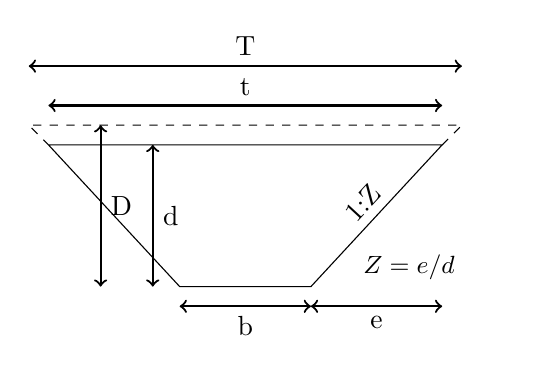
\begin{tikzpicture}[scale=1]
    \draw (\xlicho,\ylicho+\vyska) -- (\xlicho+\sirka/3,\ylicho) -- (\xlicho+\sirka/1.5,\ylicho) -- node[above,sloped] {1:Z}  (\xlicho+\sirka,\ylicho+\vyska) -- (\xlicho+\sirka,\ylicho+\vyska) -- (\xlicho,\ylicho+\vyska) ;
    \draw[dashed] (\xlicho+\sirka,\ylicho+\vyska) -- (\xlicho+\sirka+0.25,\ylicho+\vyska+0.25) -- (\xlicho-0.25,\ylicho+\vyska+0.25) -- (\xlicho,\ylicho+\vyska);
    \draw[thick,<->] (\xlicho+\sirka/3,\ylicho-0.25) --  node[below]  {b} (\xlicho++\sirka/1.5,\ylicho-0.25) ;
    \draw[thick,<->] (\xlicho++\sirka/1.5,\ylicho-0.25) --  node[below]  {e} (\xlicho+\sirka,\ylicho-0.25) ;
    \draw[thick,<->] (\xlicho+1/0.75\sirka,\ylicho) --  node[right]  {d} (\xlicho+1/0.75\sirka,\ylicho+\vyska) ;
    \draw[thick,<->] (\xlicho+0.5/0.75\sirka,\ylicho) --  node[right]  {D} (\xlicho+0.5/0.75\sirka,\ylicho+\vyska+0.25) ;
    \draw[thick,<->] (\xlicho,\ylicho+\vyska+0.5) --  node[above]  {t} (\xlicho+\sirka,\ylicho+\vyska+0.5) ;
    \draw[thick,<->] (\xlicho-0.25,\ylicho+\vyska+1) --  node[above]  {T} (\xlicho+\sirka+0.25,\ylicho+\vyska+1) ;
    \node[text width=2cm] at (\xlicho+\sirka,\ylicho+0.25){\small $Z=e/d$};
  \end{tikzpicture}} &  & & \\  
  &  &   & \\
  &  $bd + Zd^2$  & $b+2b\sqrt{1+Z^2}$  & $t = b+2dZ$ \\
  & &    & $T = b+2DZ$ \\
  &  &   & \\
  &  &  &  \\
  &  &   & \\
  &  &   & \\
  &  &   & \\
  &  &   & \\
  Trojúhelník &  &   & \\
 \multirow{2}{*}{
  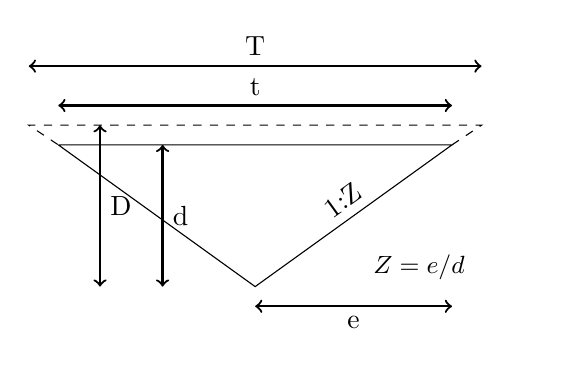
\begin{tikzpicture}[scale=1]
  % zaklad tvar
  \draw (\xtroj,\ytroj+\vyska) -- (\xtroj+\sirka/2,\ytroj) -- node[above,sloped] {1:Z}  (\xtroj+\sirka,\ytroj+\vyska) -- (\xtroj+\sirka,\ytroj+\vyska) -- (\xtroj,\ytroj+\vyska) ;
  % prirustek
  \draw[dashed] (\xtroj+\sirka,\ytroj+\vyska) -- (\xtroj+\sirka+0.375,\ytroj+\vyska+0.25) -- (\xtroj-0.375,\ytroj+\vyska+0.25) -- (\xtroj,\ytroj+\vyska);
  % d
  \draw[thick,<->] (\xtroj+1/0.75\sirka,\ytroj) --  node[right]  {d} (\xtroj+1/0.75\sirka,\ytroj+\vyska) ;
  % D
  \draw[thick,<->] (\xtroj+0.4/0.75\sirka,\ytroj) --  node[right]  {D} (\xtroj+0.4/0.75\sirka,\ytroj+\vyska+0.25) ;
  % e
  \draw[thick,<->] (\xtroj++\sirka/2,\ytroj-0.25) --  node[below]  {e} (\xtroj+\sirka,\ytroj-0.25) ;
  % t
  \draw[thick,<->] (\xtroj,\ytroj+\vyska+0.5) --  node[above]  {t} (\xtroj+\sirka,\ytroj+\vyska+0.5) ;
  % T
  \draw[thick,<->] (\xtroj-0.375,\ytroj+\vyska+1) --  node[above]  {T} (\xtroj+\sirka+0.375,\ytroj+\vyska+1) ;
  % Z
  \node[text width=2cm] at (\xtroj+\sirka,\ytroj+0.25){\small $Z=e/d$};
  \end{tikzpicture}}   &   &   & \\
  &  &   & \\
  &  $Zd^2$   & $b+2b\sqrt{1+Z^2}$   &  $t = 2dZ$ \\
  &  &  &  $T =  2  \frac{D}{d} t$  \\
  &  &   & \\
  &  &  &  \\
  &  &  &  \\
  &  &  &  \\
  &  &  &  \\
  &  &  &  \\
  Parabola &  &  &  \\
 \multirow{2}{*}{
  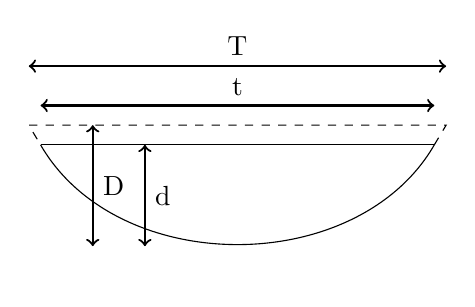
\begin{tikzpicture}[scale=1]
  \draw (\xpara,\ypara+\vyska) -- (\xpara+\sirka,\ypara+\vyska);
  \draw[dashed] (\xpara+\sirka,\ypara+\vyska) -- (\xpara+\sirka+0.15,\ypara+\vyska+0.25) -- (\xpara-0.15,\ypara+\vyska+0.25) -- (\xpara,\ypara+\vyska);
  \draw (\xpara,\ypara+\vyska) to[out=-60,in=-120] (\xpara+\sirka,\ypara+\vyska);
  \draw[thick,<->] (\xpara,\ypara+\vyska+0.5) --  node[above]  {t} (\xpara+\sirka,\ypara+\vyska+0.5) ;
  \draw[thick,<->] (\xpara-0.15,\ypara+\vyska+1.0) --  node[above]  {T} (\xpara+\sirka+0.15,\ypara+\vyska+1.0) ;
  \draw[thick,<->] (\xpara+1/0.75\sirka,\ypara+\vyska/3.5) --  node[right]  {d} (\xpara+1/0.75\sirka,\ypara+\vyska) ;
  \draw[thick,<->] (\xpara+0.5/0.75\sirka,\ypara+\vyska/3.5) --  node[right]  {D} (\xpara+0.5/0.75\sirka,\ypara+\vyska+0.25) ;
  \end{tikzpicture}}   &   &  &  \\
  &  &  &  \\
  & $\frac{2}{3}td$  & $t + \frac{8d^2}{3t} $  & $t = \frac{3A}{2d}$ \\
  &  &   &  $T = t \left(\frac{D}{d}\right)^{1/2} $ \\
  &  &   & \\
  &  &   & \\
  &  &   & \\
\end{tabular}
\end{table}


